% ==============================================================================
% SECTION 2: LINEAR MODELING & IDENTIFICATION
% ==============================================================================
\begin{frame}{System Modeling}
    \framesubtitle{Linear Model: Hammerstein Approach}
    \begin{columns}[T]
        \begin{column}{0.5\textwidth}
            \begin{block}{Static Characteristic $N(u)$}
                3rd-order polynomial identified on steady-state regimes:
                \begin{equation*}
                    v(t) = N(u) = a_3 u^3 + a_2 u^2 + a_1 u + a_0
                \end{equation*}
                \textbf{Tau identification}
            \end{block}
        \end{column}

        \begin{column}{0.5\textwidth}

                \centering
                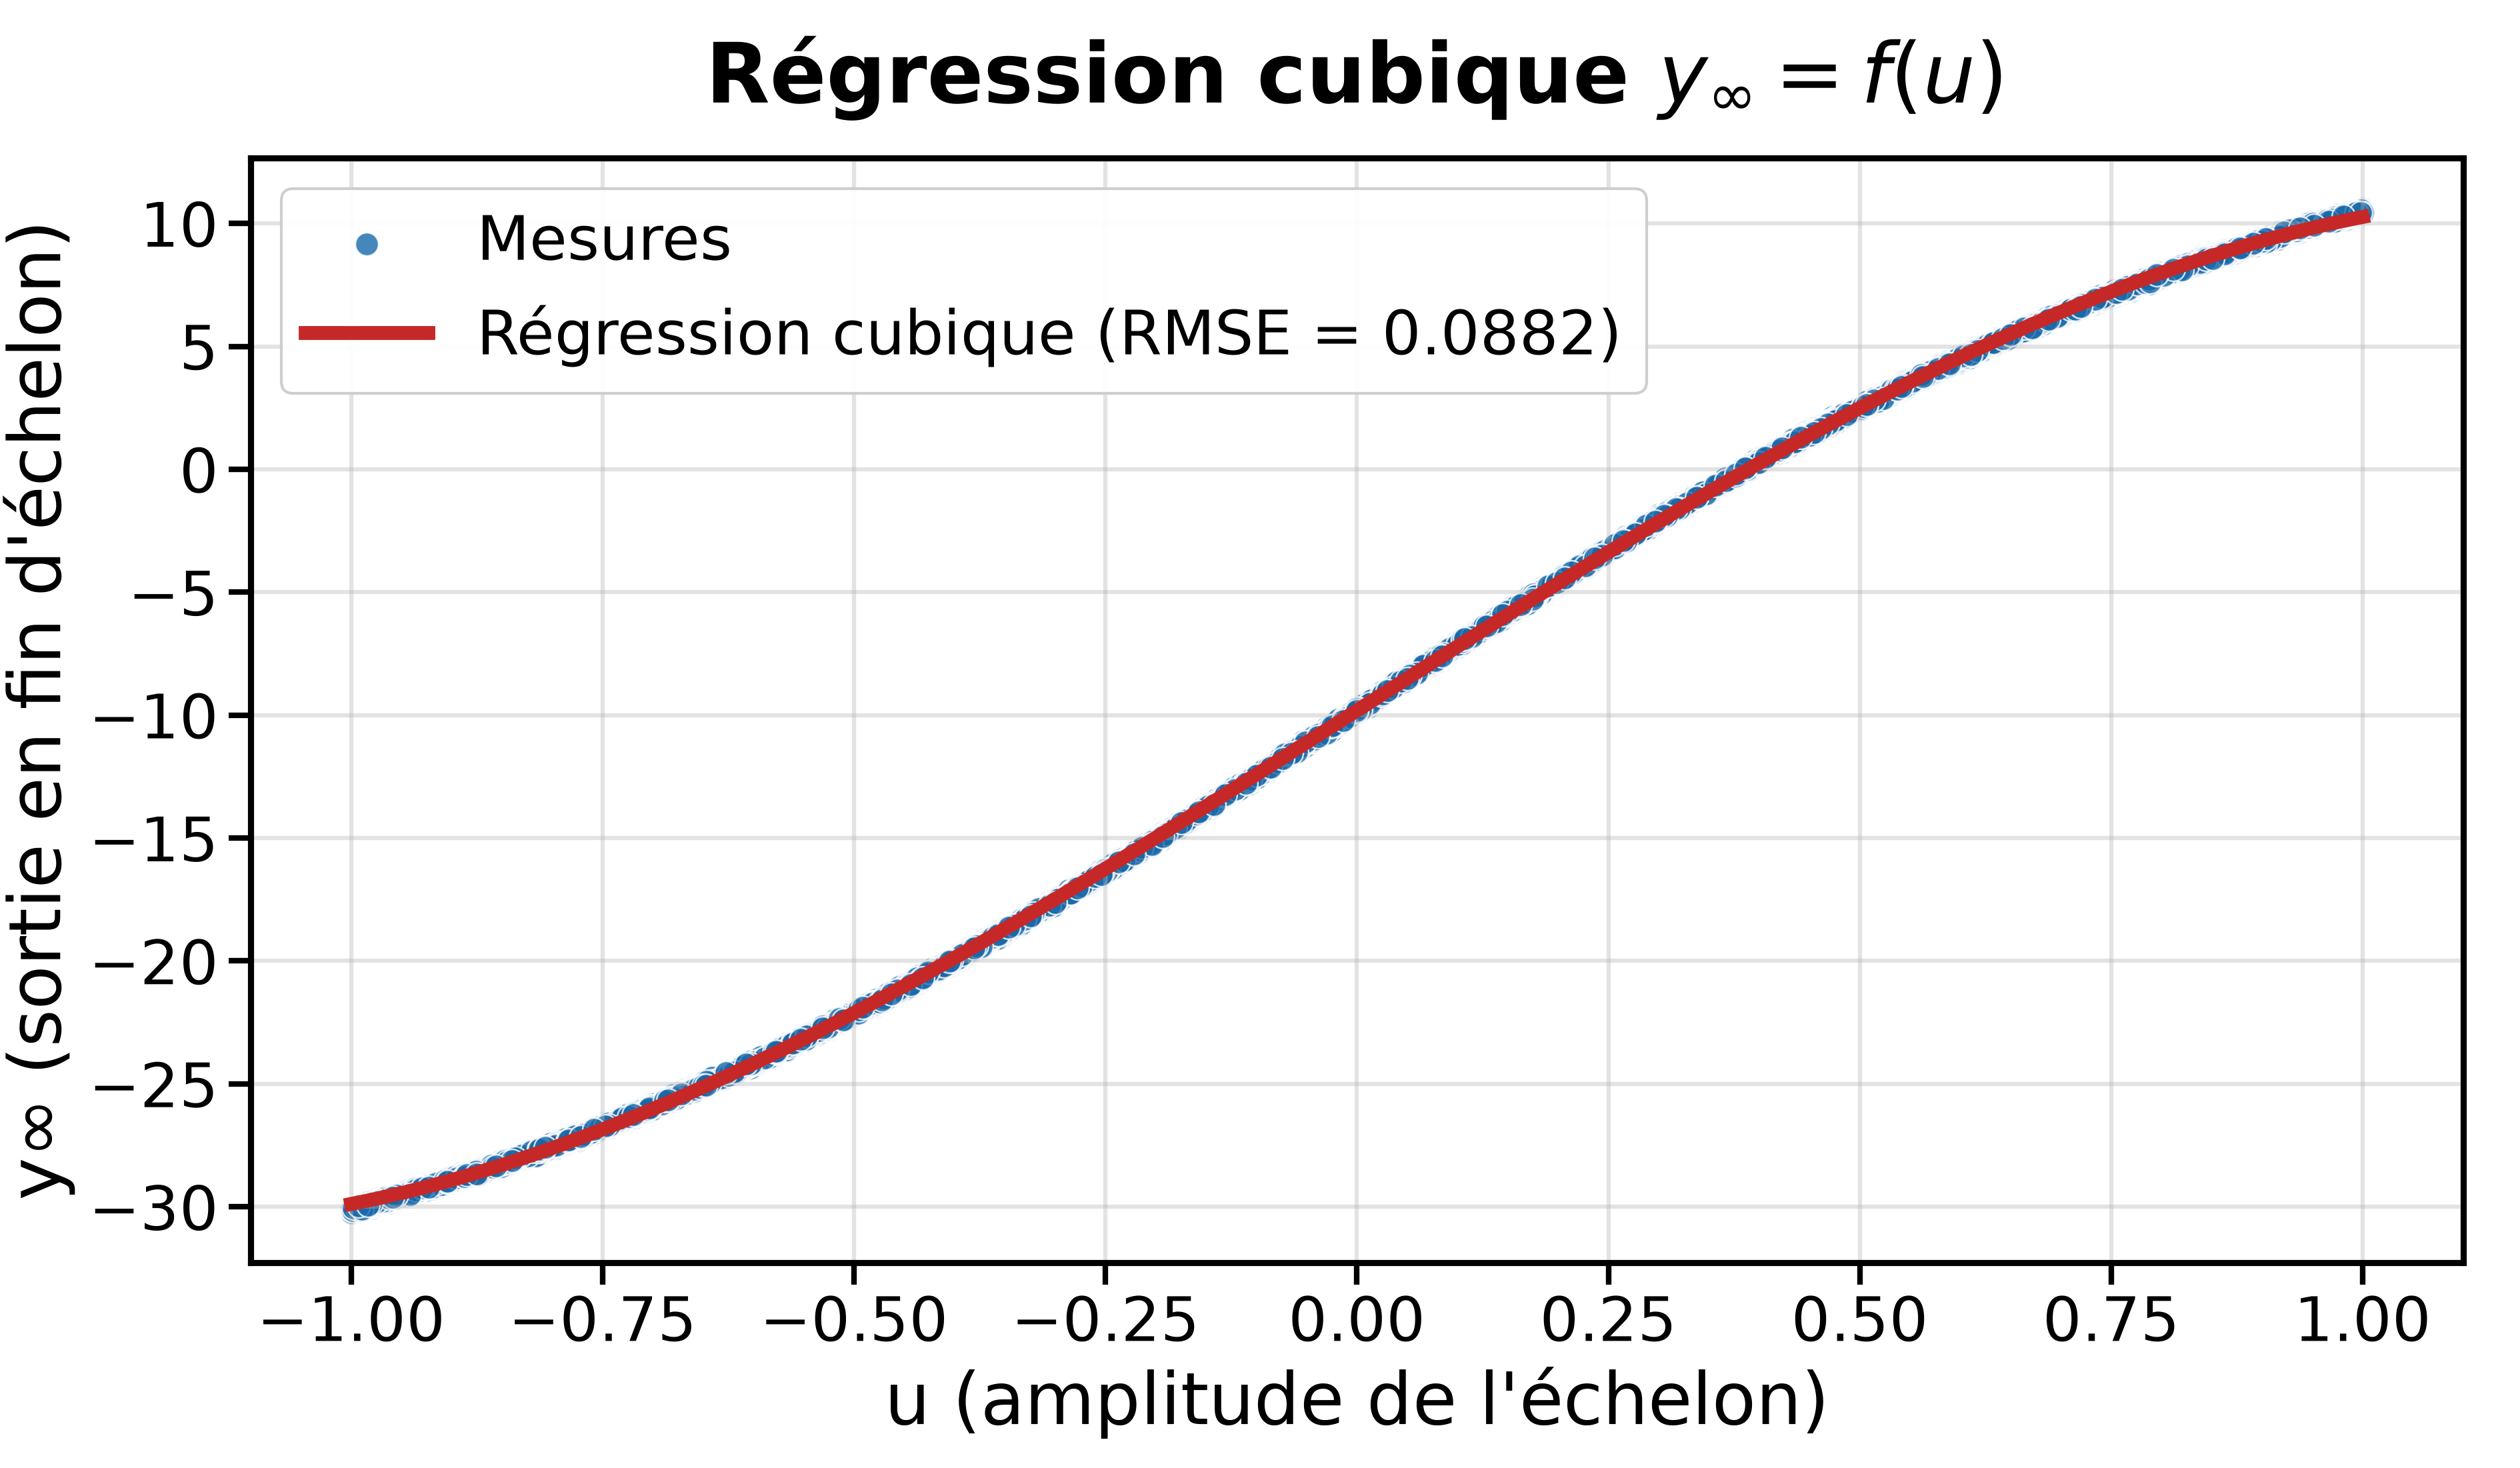
\includegraphics[
                    width=\linewidth,
                    height=2.6cm,
                    keepaspectratio
                ]{regression sur caracteristique statique.png}


                \centering
                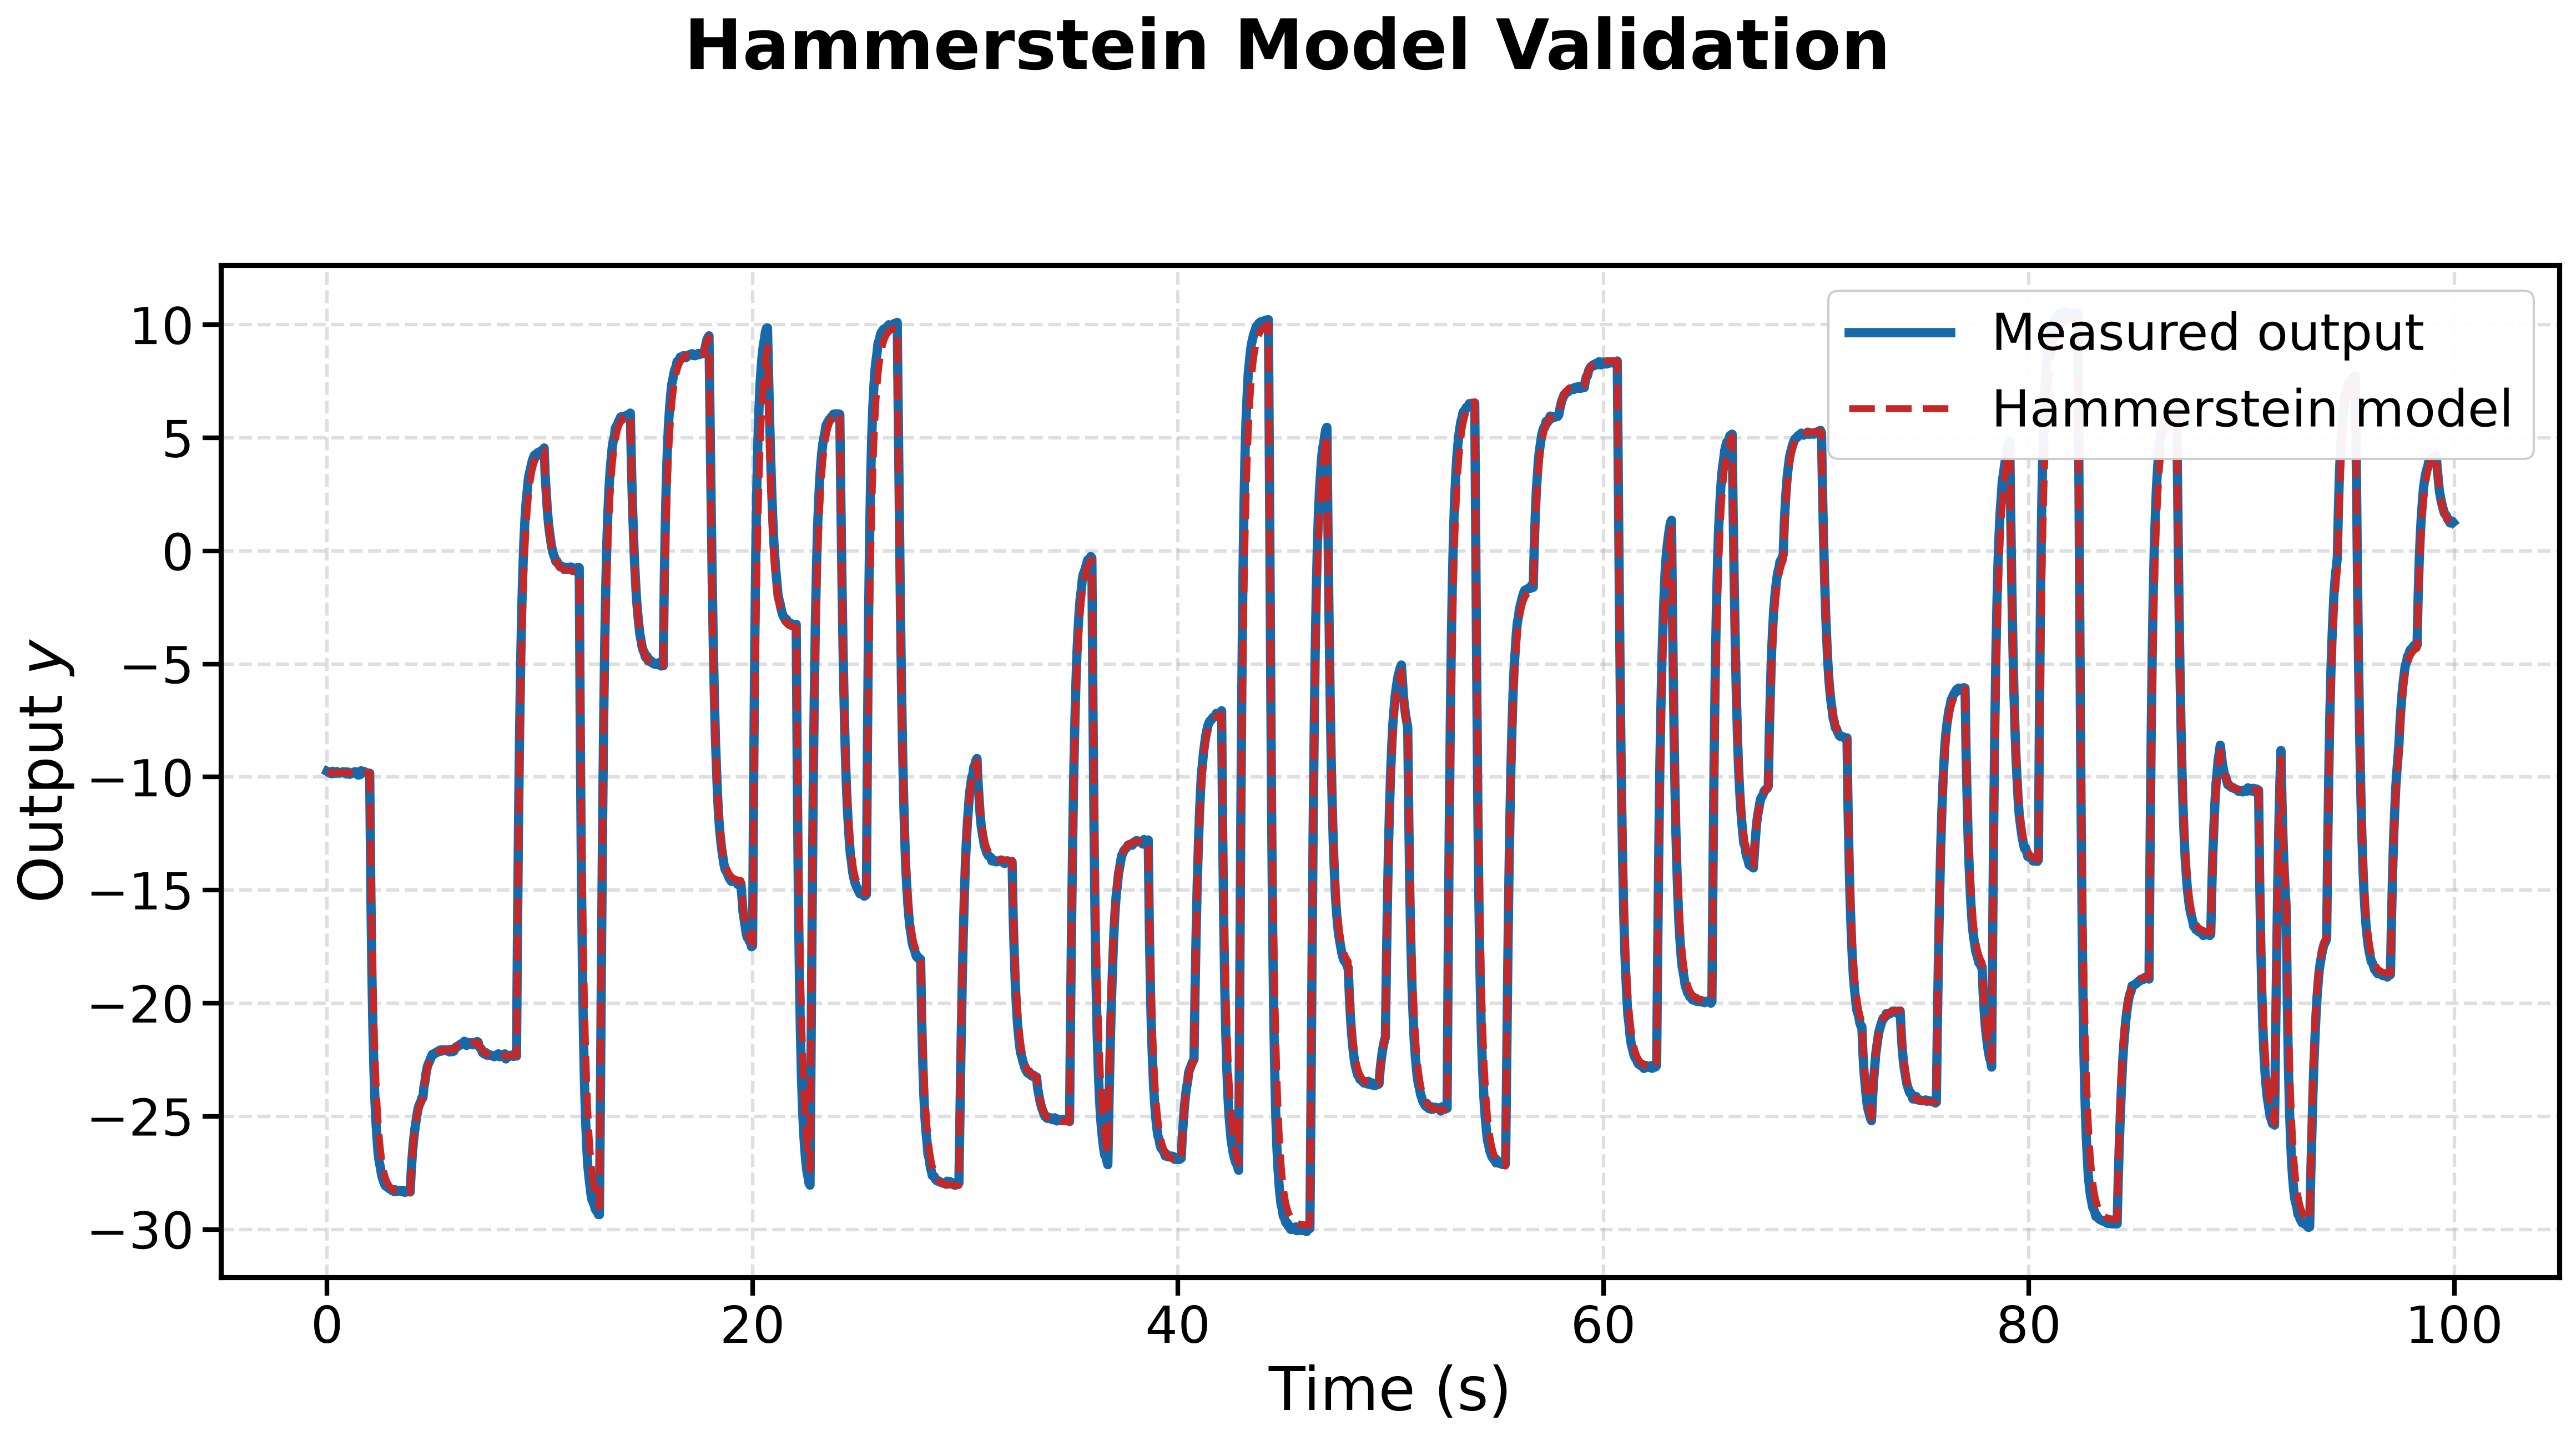
\includegraphics[
                    width=\linewidth,
                    height=5.0cm,
                    keepaspectratio
                ]{hammerstein_model_validation.png}
                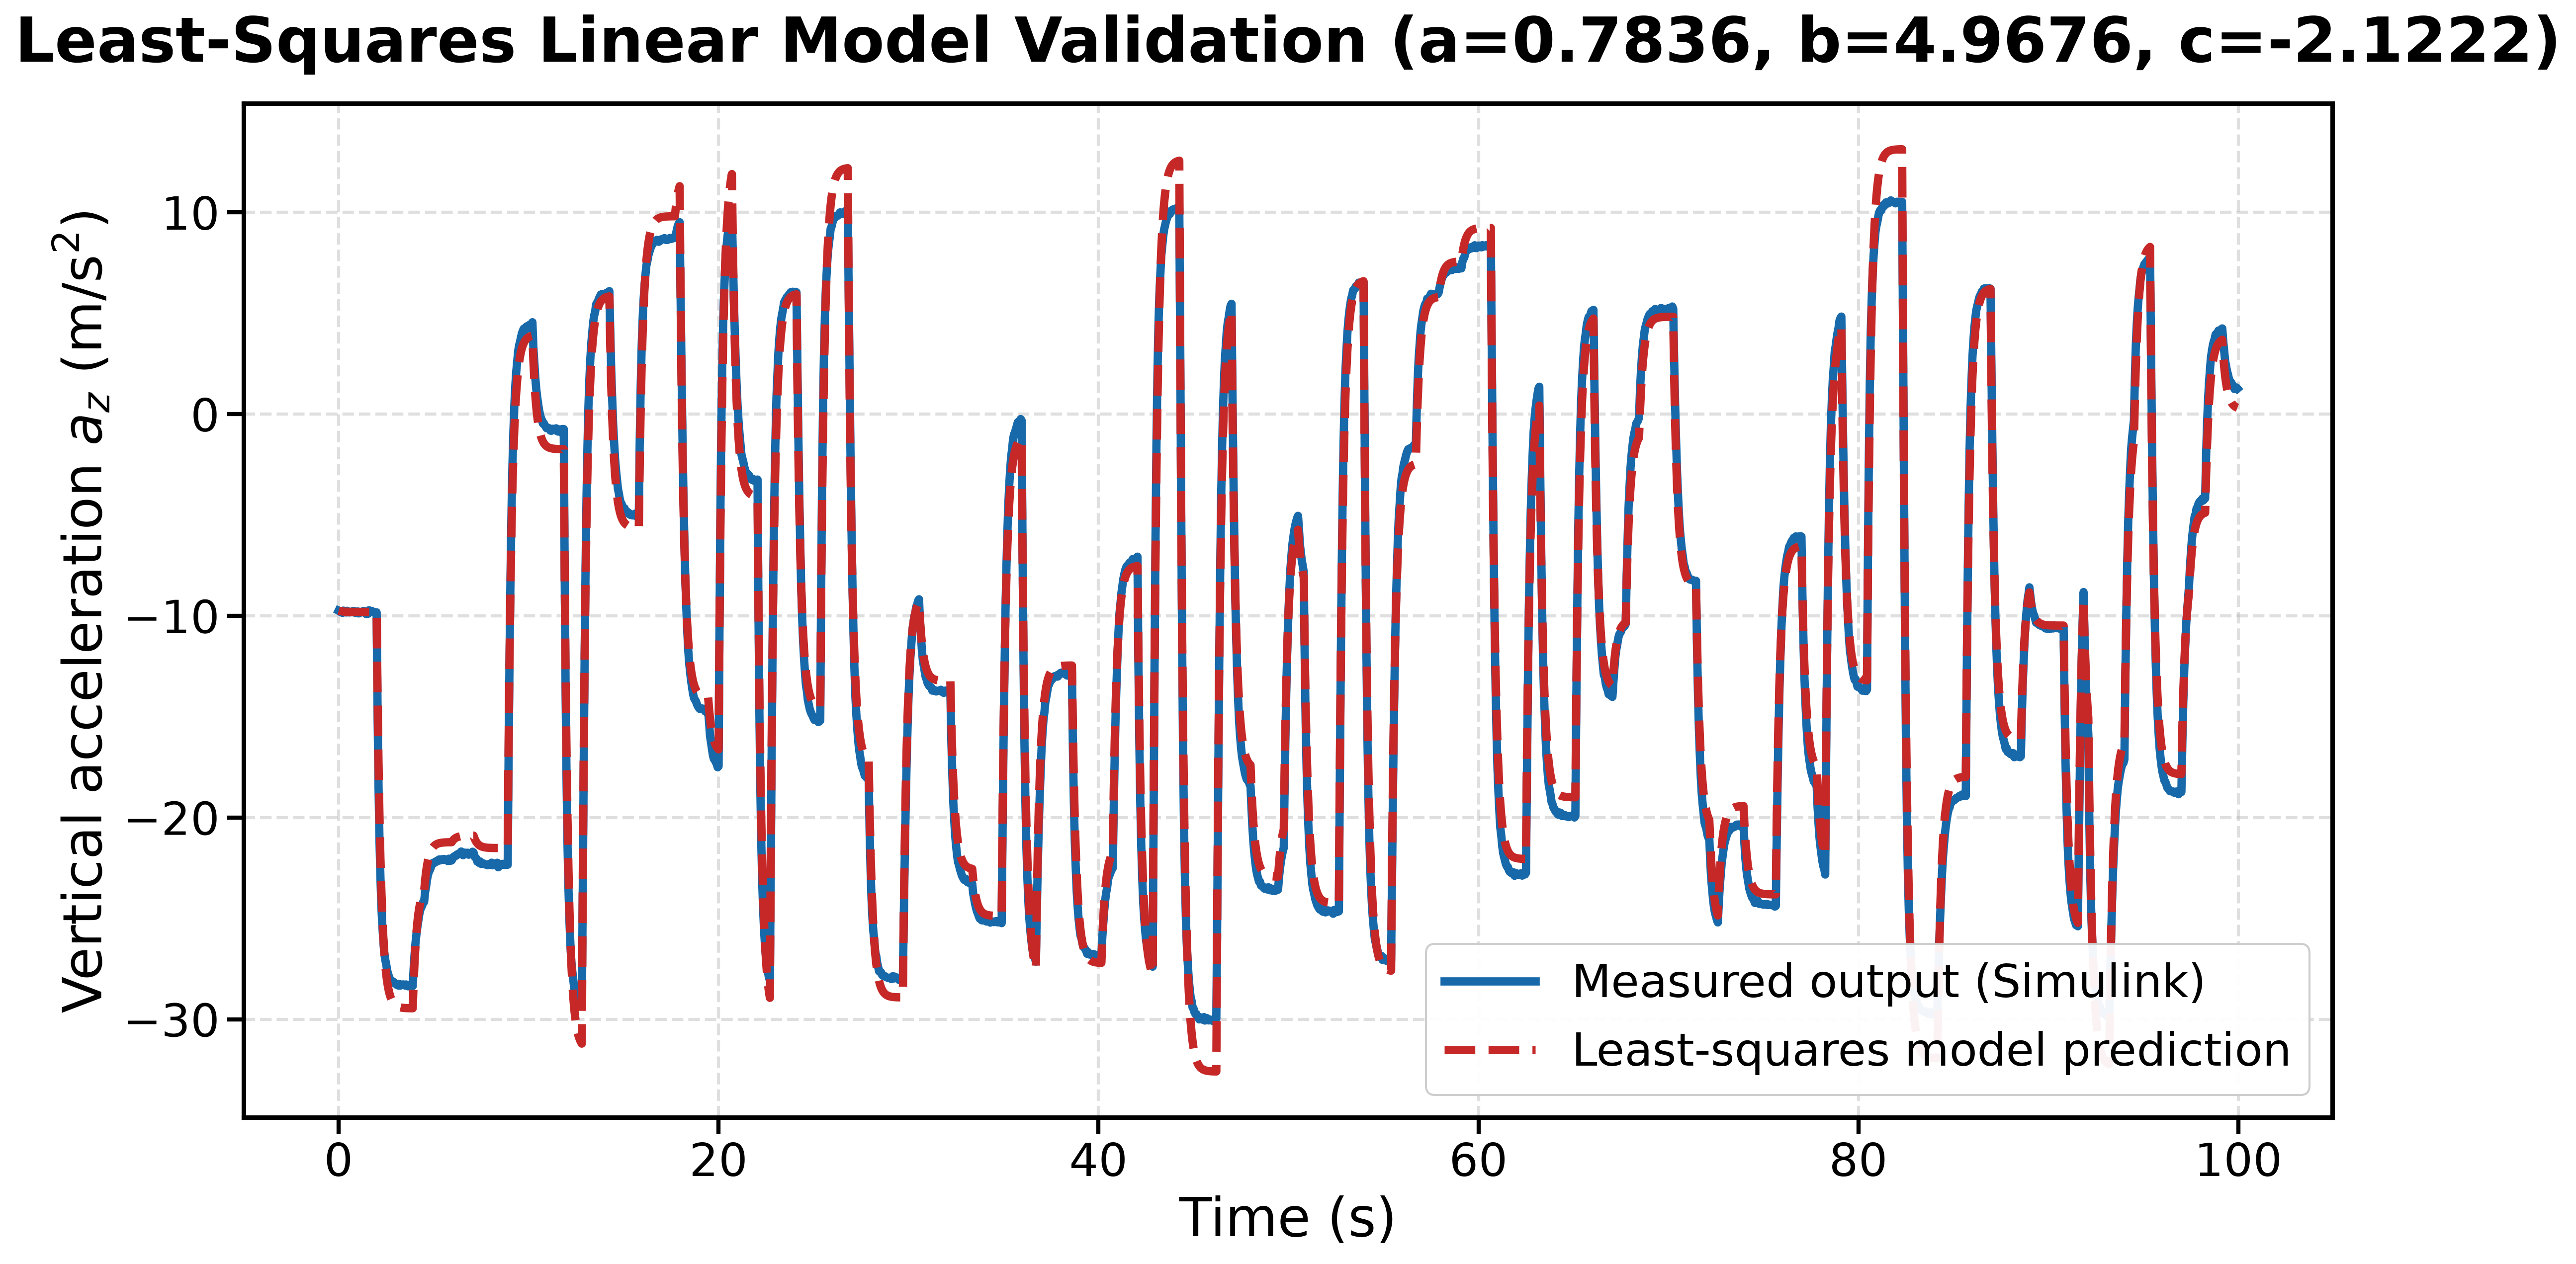
\includegraphics[
                width=\linewidth,
                height=2.75cm,
                keepaspectratio
            ]{least_squares_model_validation.png}
        \end{column}
    \end{columns}
\end{frame}

\begin{frame}{System Modeling}
    \framesubtitle{Linear Model: Least Square Method}
    \begin{columns}[T]
        \begin{column}{0.52\textwidth}

            \begin{block}{Model equations}
                \begin{align*}
                    y_k(t+1)
                        &= a\,y_k(t) + b\,u_k(t) + c \\
                        &= \boldsymbol{\varphi}_k^{\mathsf T}
                           \boldsymbol{\theta}.
                \end{align*}
                \[
                    \boldsymbol{\varphi}_k^{\mathsf T} =
                    \begin{bmatrix} y_k(t) & u_k(t) & 1 \end{bmatrix}
                    \qquad
                    \boldsymbol{\theta} =
                    \begin{bmatrix} a & b & c \end{bmatrix}^{\mathsf T}.
                \]

                The least-squares estimate is
                \begin{equation*}
                    \boldsymbol{\theta}^{\star}
                        =
                        \left(\boldsymbol{\Phi}^{\mathsf T}
                        \boldsymbol{\Phi}\right)^{-1}
                        \boldsymbol{\Phi}^{\mathsf T}\boldsymbol{Y}.
                \end{equation*}
            \end{block}
        \end{column}

        \begin{column}{0.48\textwidth}
            \centering

            \vspace{0.15cm}

            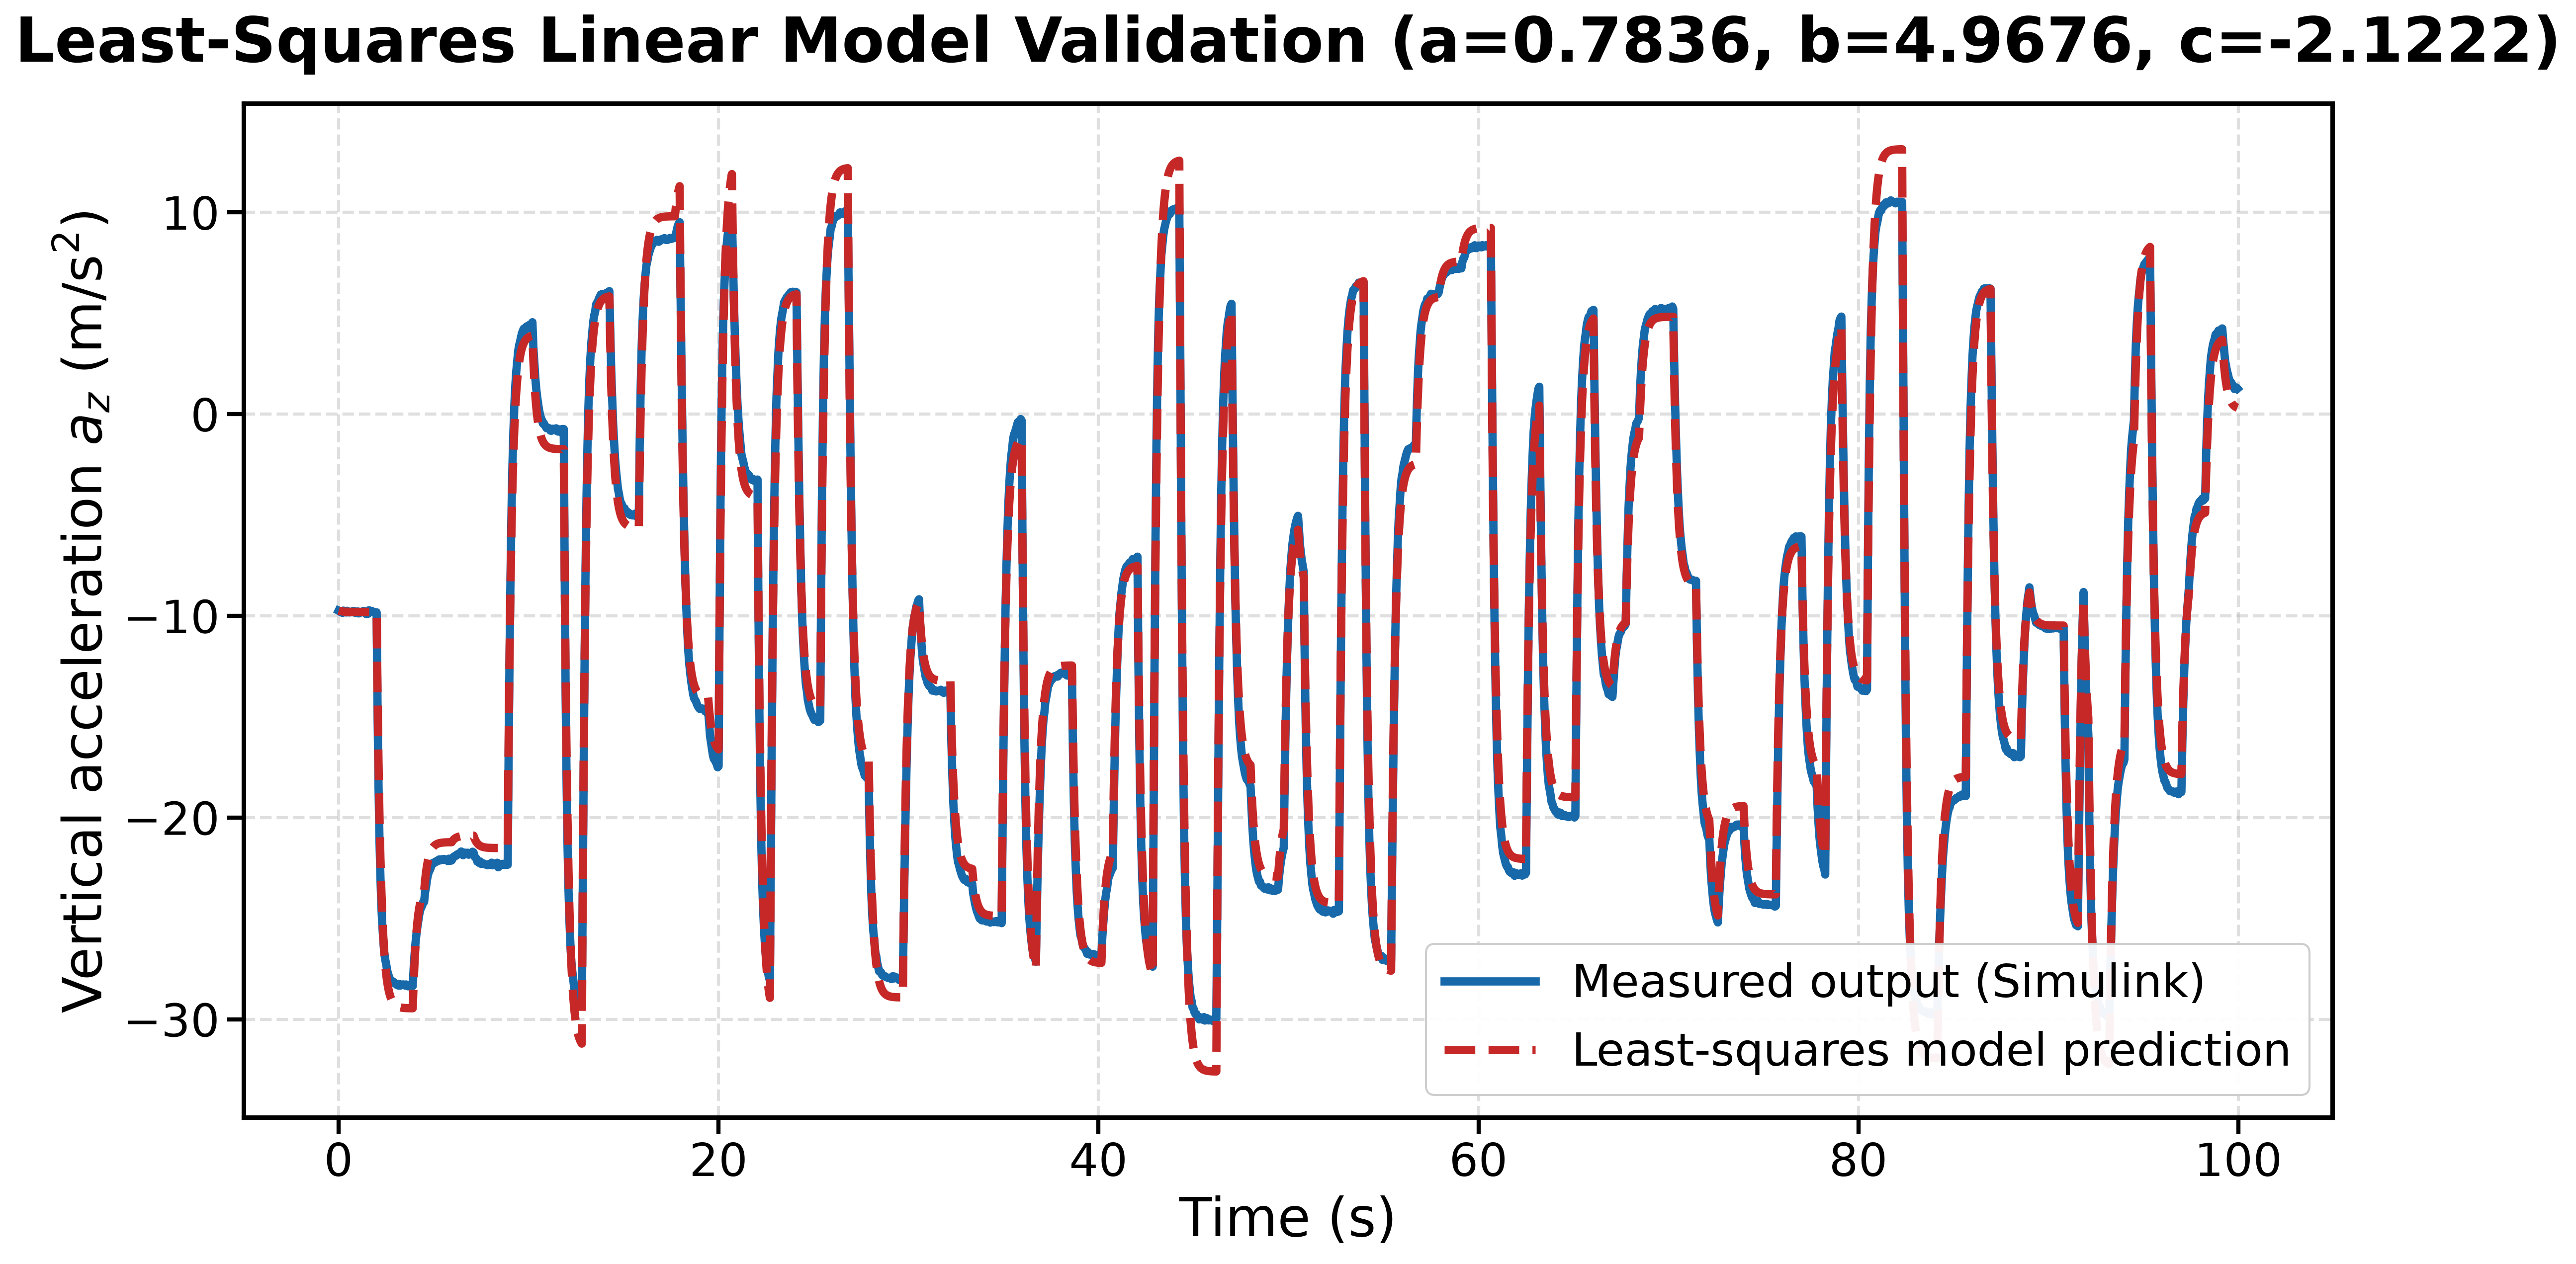
\includegraphics[
                width=\linewidth,
                height=2.75cm,
                keepaspectratio
            ]{least_squares_model_validation.png}
        \end{column}
    \end{columns}
\end{frame}
